\section{Architekturkonzept}
\label{sec:architekturkonzept}
    Das Framework stellt die Kern-Funktionalität zur Steuerung von implementierten Regeln und Prozessen innerhalb eines 
    Büroraumes dar. Diese bildet das Fundament des Systems. Das Architekturkonzept umfasst ausschließlich den 
    grundlegenden Aufbau, sowie die Funktionalitäten des Frameworks der Steuerzentrale. Potentielle Erweiterungen und 
    Adaptionen werden im Ausblick (\ref{chap:ausblick}) aufgegriffen.
    \\ 
    \linebreak
    Das System soll in drei Schichten aufgeteilt werden. Die oberste Schicht stell die Kommunikationsschicht dar, bei der mittleren 
    handelt es sich um die Logik- und Prozessschicht und die unterste repräsentiert die Persistenzschicht. Im Rahmen der Arbeit wird 
    die dritte Schicht nicht weiter behandelt, da diese zu aktuellem Zeitpunkt keinen Nutzen generiert, bzw. für keine weitere Verarbeitung 
    genutzt wird. Der Abbildung (\ref{fig:schichtenarchitektur}) ist die Aufteilung der Schichtenarchitektur zu entnehmen. In 
    der Darstellung unterscheidet sich die Persistenzschicht von den anderen, um 
    erkenntlich zu machen, dass diese nicht detailliert beschrieben wird. 
    \\
    Durch die Darstellung in übergreifender Form wird deutlich, das bereits auf dieser Ebene die Trennung der Zuständigkeiten, engl. 
    \textit{seperation of concerns}, greift. Durch die gezielte Abstraktion von Komponenten und Informationen kann die Komplexität 
    eines Systems gesteuert werden. Die Kommunikationsschicht ermöglicht die Anbindung von verschiedensten Kommunikationsprotokollen, die 
    dadurch schnell adaptiert werden können. Im Rahmen des Konzeptes wird ausschließlich Gebrauch des \acs{MQTT}-Protokolls gemacht. 
    Die Logikschicht nimmt alle eingehenden Events der Kommunikationsschicht entgegen und durchläuft den Prozess des Frameworks. Die 
    Persistenzschicht ist für die Speicherung erzeugter Daten zuständig, bspw. wenn eine Transaktionshistorie von Zustandsänderungen 
    persistiert werden soll. Ebenso können Informationen gespeichert werden, die anderweitig zur Verfügung stünden. 
    \begin{figure}[hbt!]
        \centering
        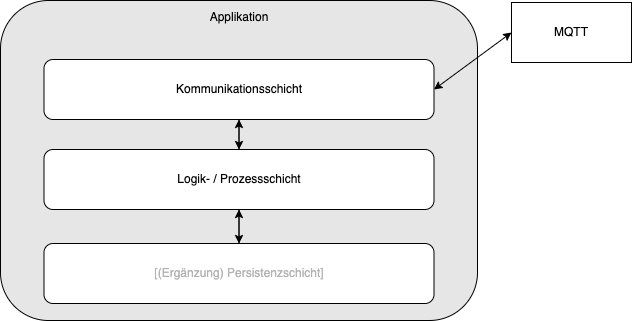
\includegraphics[width=14cm,height=10cm,keepaspectratio]{images/Schichtenarchitektur.png}
        \caption{Schichtenarchitektur}
        \label{fig:schichtenarchitektur}
    \end{figure}
    % Es wird alles abgebildet über einen Zustandsraum, der sich aus den Dingen (Gegenständen) und Zuständen der Anwendung ergibt.
    % Der Zustandsraum wird verändert, wenn eine Aktion durchgeführt wird, bzw. durch eine Trigger angestoßen. 
    % Bzw. speichert den aktuellen Zustand des Gegenstandes 
    % (lightBulb = true/false, personOnDoor = null/Mikka, booking = stringBooking, temiAktive = true/false, 
    % temiPosition = stringKoordinates)
    % Zustandsraum muss von dem Entwickler definiert werden. 
    % MQTT Broker über Home Assistant, bzw. losgelöster Broker
    % Anbindung von APIs auch Entwickler-Sache. Kann ich das vereinfachen, sodass die Integration einfacher wird?

    \subsection{Überlegungen, Anstöße und Herausforderungen}
    % Regeln über Thread abbilden? Ja, Nein? - Nein, wieso? Da Durch die MQTT Message mehrere Regeln ausgeführt 
    %werden können. -> Lediglich den Zustand der Komponenten locken.
    % KEIN THREAD (wird schon abgebildet durch die Services und die Auslöser durch MQTT), Falls eine Komponente 
    %  doppelt beansprucht wird, ist der Zustand der Komponenten zu locken und ein 
    % Thread.sleep einzurichten. Abfrage, ob der Wert, bzw. die Komponente wieder freigegeben wurde. 

    % Zustandsraum -> Abbildung aller notwendigen Komponenten 
    % Bei Bearbeitung einer Regeln die Komponenten Locken, sodass nur die einzelne Komponenten (deren Zustand) gelockt ist 
    % und nicht der ganze Zustandsraum, somit können mehrere Komponenten und Aktionen ausführen zu können. 

    %Was brauche ich für Funktionen und Werte in einer Regel?

    % Ein Zustandsraum (Objekt) für alles oder ein Globales, welches die die Komponenten enthält? - Begründung für die Auswahl.
    
    %\subsection{Schnittstellen}
        % Kommunikation mit API's je nach Use Case und Gebrauch zur Datenabfrage
    
    %\subsection*{Datenbanken}
    %   Anbindungen an Datenbanken sind je nach hinzukommendem Anwendungsfall ohne weiteres möglich. Dies ist eine Konzeptvertiefung, die 
    %    im Rahmen dieser Arbeit nicht konkretisiert wird, da der Fokus auf der Kernfunktionalität, sowie auf dem 
        % Datenbanken je nach Use Case und Gebrauch zur Datenabfrage


    %HERAUSFORDERUNG MIT DEM QUEUEING ANTEASERN.

\subsection{Softwarekonzept}
\label{subsec:softwarekonzept}



